\chapter{Srovnání nástrojů}
Pro srovnání nástrojů jsem vytvořil návrh multikriteriálního hodnocení, který se snaží nástroje hodnotit z~různých úhlů a~vytvořit tak komplexní klasifikaci. Každé z~hodnocených částí je možné přiřadit vlastní váhu. Ta určuje důležitost hodnotícího kritéria pro každého jedince a~tím napomáhá výběru vhodného nástroje. V~obrázku \ref{MKHodn} je návrh ukázán a~je vidět výsledek pro mnou zvolené váhy, viz obrázek \ref{MKVysl}. Jako nejvhodnější se jeví použití nástroje SikuliX. Dále se budu věnovat jednotlivým hodnotícím kritériím.

Možnost vytváření skriptů je jedno z~nejdůležitějších kritérií vzhledem k~vazbě na předmět KIV/OKS. Hlavním požadavkem bylo, aby bylo možné skripty tvořit v~jazyce Java. Dále jsem vybral několik skriptovacích jazyků a~metod.

Podpora testovaných rozhraní byla dalším z~rozhodujících kritérií. Hlavními platformami měly být aplikace vytvořené pomocí jazyka Java a~webové aplikace. Opět jsem přidal některé další běžné platformy. Nástroj by měl být též multiplatformní, proto je jedním z~kritérií podpora operačních systémů.

Reportování výsledků testů, složitost jejich tvorby a~jejich přehlednost může napomoci vývojáři diagnostikovat případnou chybu. Také je přínosné znát stav obrazovky a~to zajistí screenshot. Díky tomu se stává vývoj jednodušší, a~proto jsem toto kritérium také zařadil do hodnocení.

Dále jsem přidal kritérium univerzálnosti nástroje s~poněkud individuálním ohodnocením. To je zde myšleno tak, co obecně nástroj dokáže, ale co není podstatné z~pohledu předmětu KIV/OKS. Například Jubula je čistě testovací nástroj, ale SikuliX se dá použít navíc pro automatizaci pracovních postupů.

Posledním kritériem je vhodnost nástroje pro účely předmětu KIV/OKS. Jedná se hlavně o~to, jak zapadá do konceptu výuky, jak je práce s~ním složitá a~jaké má nároky na studentovy znalosti.

Vysvětlivky termínů z~dále použitých tabulek:
\begin{itemize}
	\item Natural-like -- víceméně okleštěný přirozený jazyk založený na angličtině,
	\item Složitost tvorby -- míní se tím složitost přípravy reportu a~v~tabulce vyšší počet bodů znamená jednodušší tvorbu pro tvůrce skriptů
\end{itemize}
\begin{figure}[ht!]
	\begin{subfigure}{\textwidth}
		\centering
		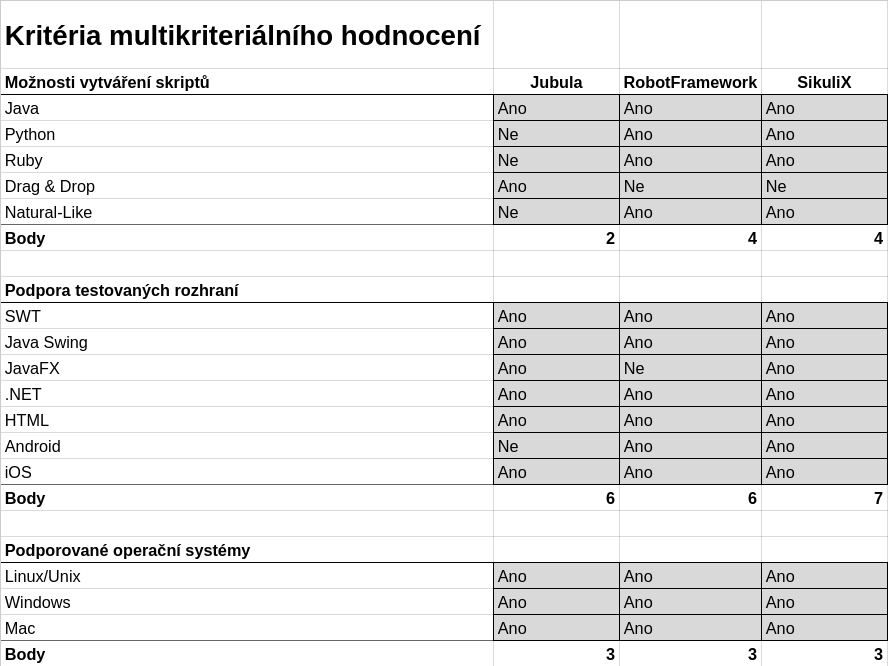
\includegraphics[width=13.5cm]{img/Kriteria/Kriteria1.png}
		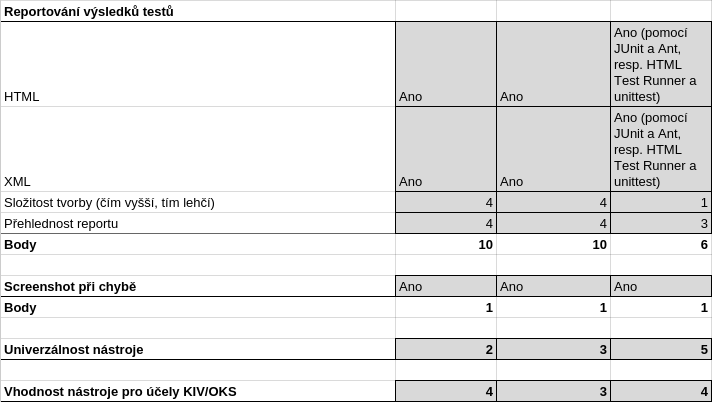
\includegraphics[width=13.5cm]{img/Kriteria/Kriteria2.png}
		\caption{Multikriteriální hodnocení}
		\label{MKHodn}
	\end{subfigure}
\end{figure}
\begin{figure}[ht!]
	\ContinuedFloat
	\begin{subfigure}{\textwidth}
		\centering
		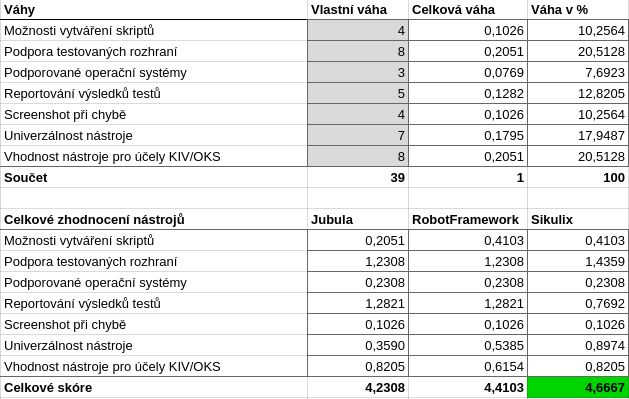
\includegraphics[width=13.5cm]{img/Kriteria/Kriteria3.png}
		\caption{Výsledek multikriteriálního hodnocení}
		\label{MKVysl}
	\end{subfigure}
\end{figure}

Z~uvedeného multikriteriálního hodnocení je zřejmé, že vybrané nástroje jsou v~podstatě vyrovnané. To ostatně potvrzuje i~jejich poměrné zastoupení mezi uživateli. SikuliX byl zvolen též po diskuzích s~vedoucím práce a~to pro jeho vlastnost naprosté nezávislosti na testovaném rozhraní. Tato vlastnost se významně hodí v~předmětu KIV/OKS, protože je možné dát nástroj do kontrastu s~nástrojem Selenium. Jinými slovy řečeno SikuliX je principiálně odlišný nástroj, což není možné říci o~např. Jubule.